\label{sec:man}
%%%%%%%%%%%
In this section a user manual is presented. The section starts with a general overview of the code
organisation and it follows with a more detailed explanation for the most frequently used functions.

%%%%%%%%%%%%%%%%%%%%%%%%%%%%%%%%%%%%%%%%
\subsubsection{Code Organisation}
A general diagram of  available modules is illustrated in figure~\ref{fig:org}.
The flow is depicted such that it follows the structure of the \fitter\ .
\begin{figure}
\begin{center}
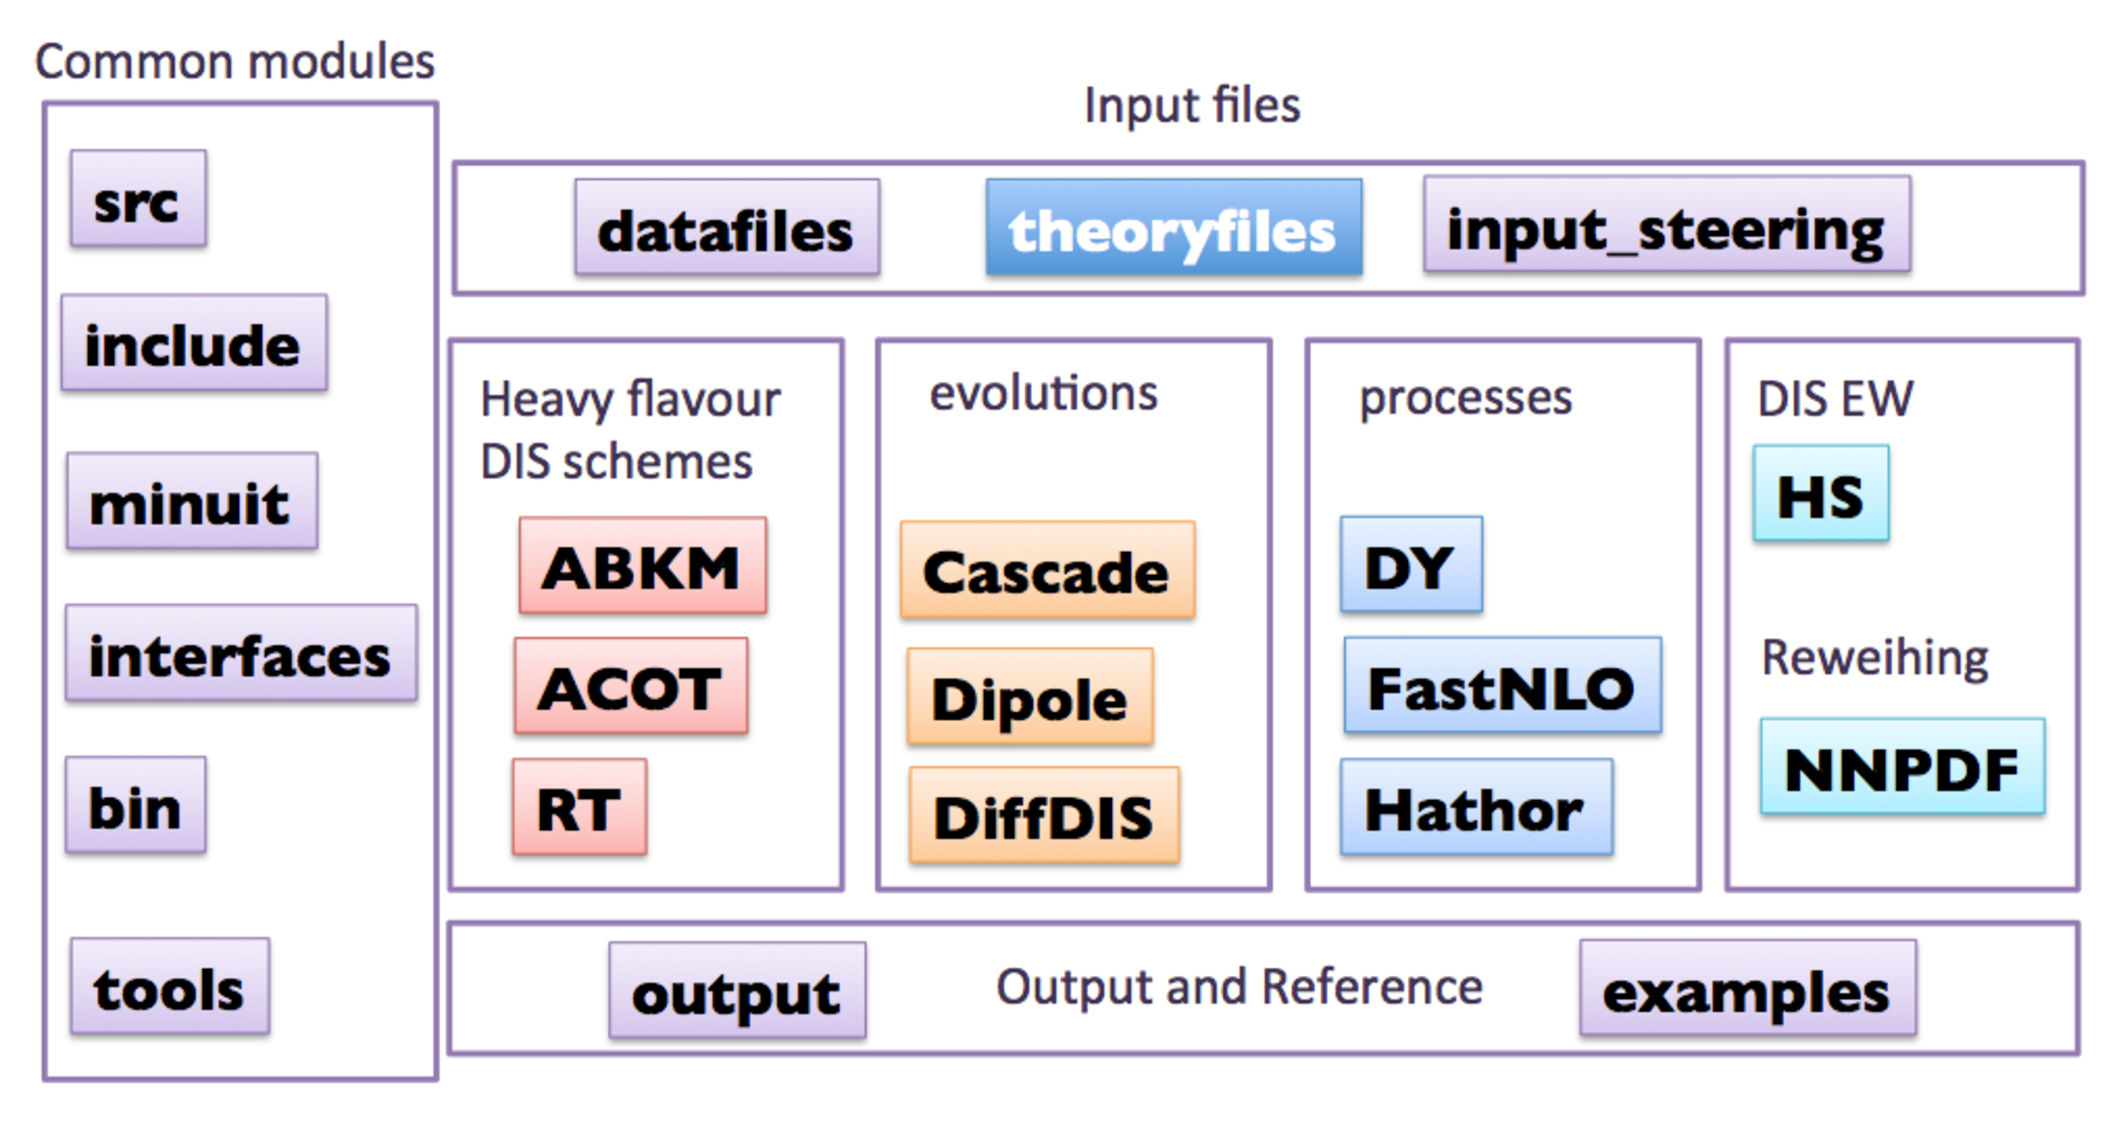
\includegraphics[width=0.75\linewidth]{figures/organisation.pdf}
\end{center}
\caption{Schematic structure of the \fitter\ program organisation in different modules.}
\label{fig:org}
\end{figure}

In addition, an inventory list with short description of existing subroutines is  
presented in Table~\ref{tab:list}. 
Here we choose to enlist only the routines from the common target module to guide 
the user of available functionalities.

\begin{center}
\begin{table}
\begin{tabular}{lp{4cm}p{10cm}}
\hline
\hline
\small\bf{steerings} & $\bullet$ steering.txt:& free PDF parameters to be varied by MINUIT \\
 & $\bullet$ minui.in.txt:& main steering card \\
 & $\bullet$ ewparam.txt:& settings of electroweak parameters, as well as masses \\
\toprule
\bf{src} & $\bullet$ main.f:& main program \\
& $\bullet$ read\_steer.f: &access steer parameters from steering card \\
& $\bullet$ read\_data.f: & reading the datatables and storing data information \\
& $\bullet$ init\_theory.f: & initialising theory modules \\
& $\bullet$ dataset\_tools.f:&  allocating bin indices \\
& $\bullet$ error\_logging.f: &  error logging information\\
& $\bullet$ minuit\_ini.f: & initialise minuit module \\
& $\bullet$ fcn.f: & passes to minuit the $\chi^2$ to be minimised \\
& $\bullet$ pdf\_param.f:  &  parametrisation of the PDFs at starting scale\\
& $\bullet$ sumrules.f: & PDF constraints at starting scale, such as QCD sum rules. \\
& $\bullet$ evolution.f: & evolution of PDFs \\
& $\bullet$ theory\_dispatcher.f: & distribution of theory prediction calculations for a given dataset  \\
& $\bullet$ dis\_sigma.f & calulates the DIS cross sections \\
& $\bullet$ GetChisquare.f & calculates the $\chi^2$  \\
& $\bullet$ GetCovChisquare.f & calculates the $\chi^2$ using covariance matrix \\
& $\bullet$ GetPointScaledErrors.f & calculates the rescaled statistical, uncorrelated and constant errors \\
& $\bullet$ prep\_corr.f & prepare systematic correlation matrix \\
& $\bullet$ systematics.f & build the matrix for systematic uncertainties and invert it \\
& $\bullet$ error\_bands\_pumplin.f  & Hessian error calculations  \\
& $\bullet$ mc\_errors.f & MC method for creating replicas of data through smearing. \\\cmidrule{2-3}
& $\bullet$ GetDiffDisXsection.f  & calulates the diffractive DIS cross sections \\
& $\bullet$ FixModelParams.f  & used for diffractive DIS cross sections \\\cmidrule{2-3}
& $\bullet$ lhapdf\_dum.f   & \tiny (used only with ENABLE\_LHPDF)\\
& $\bullet$ reweighting.f & main subroutine for PDF rewighting \tiny (used only with ENABLE\_NNPDF) \\
& $\bullet$ nnpdfreweighting.f & main subroutine for NNPDF rewighting \tiny (used only with ENABLE\_NNPDF) \\\cmidrule{2-3}
& $\bullet$ dy\_cc\_sigma.f  & calulates the DY cross sections \\
& $\bullet$ applgrids\_dum.f    & protective file against miss-use of flags in steering\\
& $\bullet$ fappl\_grid.cxx  &  \tiny (used only with ENABLE\_APPLGRID) \\
& $\bullet$ applgrids.f    &  passing PDFs to APPLGRID \tiny (used only with ENABLE\_APPLGRID) \\
& $\bullet$ pp\_jets\_applgrid.f   & calulates $pp$ jets cross sections  \\
& $\bullet$ ep\_jets\_fastnlo.f  &  calulates $ep$ jets cross sections \\\cmidrule{2-3} 
& $\bullet$ getncxskt.f  & access the NC cross sections grids for uPDFs\\
& $\bullet$ Getgridkt.f & acess the grids for uPDFs \\\cmidrule{2-3}
& $\bullet$  ttbar\_hathor\_dum.f  & protective file against miss-use of flags in steering\\
& $\bullet$  ttbar\_hathor.f  & \tiny ( used only with ENABLE\_HATHOR) \\\cmidrule{2-3}
& $\bullet$ offset\_fns.f & collects results from Offset method and stores them\\
& $\bullet$  g\_offset.cc  & file used for Offest method\\
& $\bullet$  matrix.cc  & inversion of matrix as used for Offset method \\
& $\bullet$  FitPars\_base.cc  & file used for Offest method\\
& $\bullet$  FTNFitPars.cc   & file used for Offest method\\
& $\bullet$  Xstring.cc   & file used for Offest method\\
& $\bullet$  decor.cc   & file used for Offest method\\\cmidrule{2-3}
& $\bullet$ store\_output.f & write the output  \\
& $\bullet$ store\_h1qcdfunc.f & store structure functions   \\
\bottomrule
\end{tabular}
\caption{A list of main subroutines are listed with a short description of their function.}
\label{tab:list}
\end{table}
\end{center}

%%%%%%%%%%%%%%%%%%%%%%%%%%%%%%%%%%%%%%%%
\subsubsection{Steering files}
 The software behavior is controlled by three files with steering commands.
 These files have predefined names:
    
\begin{itemize}
      \item {\tt steering.txt}  --   controls main "stable" (un-modified during 
                         minimisation) parameters. The file also contains
                         names of data files to be fitted and definitions 
                         of kinematic cuts                              
      \item {\tt minuit.in.txt}
                   --  controls minimisation parameters and minimisation 
                         strategy. Standard Minuit commands can be provided
                         in this file
      \item {\tt ewparam.txt}    --  controls electroweak parameters such
        as W and Z boson masses and CKM matrix parameters.
\end{itemize}


%%%%%%%%%%%%%%%%%%%%%%%%%%%%%%%%%%%%%%%%

\begin{description}
\item \bf{Steering.txt}\rm 

Different options are activated via steering flags in the main steering file.
%and the default steering file is displayed in figure  \ref{fig:steering}.
 
The format of the steering file follows standard "namelist" conventions.
Comments start with exclamation mark (similarly used for data file format).
The following namelist blocks are encountered:
\begin{itemize}
\item  {\tt InFiles}: Namelist to control input data
\item  {\tt InCorr}: Namelist to control statistical correlation files
\item  {\tt Scales} (Optional): Namelist to modify renormalisation/factorisation scale
\item  {\tt HeraFitter}: Main steering cards. 
%Further details can be found in the appendix \ref{sec:herafitter}. 
\item  {\tt ExtraMinimisationParameters}:  Namelist to add extra to minuit parameters.
\item  {\tt Output}: Namelist that outputs steering cards 
\item  {\tt Cuts}: Namelist for process dependent cuts
\item  {\tt MCErrors} (Optional):Namelist for MC errors steering cards
\item  {\tt Cheb} (Optional): Chebyshev study namelist
\item  {\tt Poly} (Optional): pure polynomial parameterisation for valence quarks
\item  {\tt HQScale} (Optional): choose the factorisation scale for HQs
\item  {\tt lhapdf} (Optional):LHAPDF steering card
\item  {\tt reweighting} (Optional): reweighting steering cards
\end{itemize}

These namelist blocks are described in greater details in the User's example \ref{section:example}. 


\begin{description}
\item \it\bf Theory type: \rm\\
 
here is a steering flag which defines the theory type via the chosen evolution.
The following types are supported:
\begin{itemize}
\item \tt{TheoryType = 'DGLAP' }\rm as used for collinear evolution theories. For this type another 
 flag is needed to specify the order of the perturbative series in $\alpha_S$:
\tt{Order}\rm which can be leading order (LO), next-to-leading order (NLO) and when available NNLO.
\item \tt{TheoryType = 'DIPOLE' }\rm as used for the dipole models;
\item \tt{TheoryType = 'uPDF' }\rm as used for the un-integrated PDFs (with 3 variants)
\end{itemize}

\item \it\bf Starting scale: \rm\\
The evolution starting scale is set via flag  \tt{Q02}\rm, commonly set below charm threshold, as imposed by QCDNUM.

\item \it\bf Scheme type: \rm\\
For the DIS process, several schemes are available for heavy quark treatments via  \tt{HF\_SCHEME}\rm flag.
\begin{itemize}
  \item VFNS (Variable Flavour Number Schemes):
    \begin{itemize}
     \item RT-VFNS  schemes                               [from Robert Thorne], \tt{HF\_SCHEME = RT, RT OPT}\rm, as well as the fast variants based on k-factors \tt{RT FAST, RT OPT FAST}
     \item Zero Mass VFNS                                 [qcdnum], \tt{ZM-VFNS}\rm   
     \item  ACOT (ACOT-Full, ACOT-ZM, S-ACOT-Chi) schemes  [from Fred Olness], \tt{HF\_SCHEME = ACOT Full, ACOT Chi, ACOT ZM}\rm, they are all based on k-factors. 
    \end{itemize}
  \item FFNS (Fixed Flavour Number Scheme)
    \begin{itemize}
    \item via QCDNUM, \tt{HF\_SCHEME = FF}\rm 
    \item via ABM (openqcdrad-1.6)   [from Sergey Alekhin], \tt{HF\_SCHEME = FF ABM}\rm
    \end{itemize}
\end{itemize}
IMPORTANT to note if running with FFNS (nf=3): 
\begin{itemize}
  \item only neutral current DIS data should be used in FF scheme due to missing NLO 
    coefficient functions in charged current process, in this cases valence quark parameters  
    need to be fixed in minuit.in.txt file.
  \item In FF ABM implementation the charged current coefficients are available
    therefore valence parameters do not need to be fixed.
  \item $\alpha_s(Q^2)$ in FFNS is 3-flavour and recommended to be set to the value of 0.105 
    such that is not too high at low energies
  \item the scale in FFNS is defined as $\mu^2 = Q^2 + 4m_h^2$ by default, can be 
    changed in HQScale in \tt{steering.txt}\rm (scale variation in ABM not yet implemented)
  \item  the pole mass definition for heavy quarks is set in ABM by default, 
    the running mass definition \cite{Alekhin:runm} can be switched in 
    by setting \tt{HF\_SCHEME = FF ABM RUNM} \rm in \tt{steering.txt} \rm. 
\end{itemize}

\item \it\bf PDF parametrisation style: \rm\\
There are various types of parametric functional form supported by \fitter\ .
They are accessed via the steering flag called \tt{PDFStyle}\rm. Available styles
are summarised as follows:

\begin{tabular}{ll}
 \tt  '10p HERAPDF'   & -- HERAPDF-like with extra assumption Buv = Bdv \\
 \tt   '13p HERAPDF' & -- HERAPDF-like with Buv and Bdv floated independently and two fur-\\
                     &  ther free parameters for the gluon PDF which allow it to be negative at \\
                     &  low scale\\
 \tt   '10p H12000'  & -- H12000-like (D,U,Dbar,Ubar+g) \\
 \tt   'CTEQ'        & -- CTEQ-like parameterisation \\
 \tt   'CHEB'        & -- CHEBYSHEV parameterisation based on glu, sea, uval, dval evolved\\
                     &  pdfs \\
 \tt  'LHAPDFQ0'    & -- use lhapdf library to define pdfs at starting scale and evolve with local \\
                    &  qcdnum parameters \\
 \tt  'LHAPDF'      & -- use lhapdf library to define pdfs at all scales\\
 \tt   ' DDIS'        & -- use Diffractive DIS \\
 \tt  'BiLog'       & -- bi-lognormal parametrisation \\
\end{tabular}


These styles were described in details in section~\ref{sec:pdfparam}.
The LHAPDF style can be used only with proper configuration settings,
 as explained in the section~\ref{sec:install}.
\item \it\bf  Definition of Chisquares:\rm\\
Currently two different formats of defining $\chi^2$ are supported.
The new format is explained in the section \ref{sec:chi2}.
%Currently two different styles are supported for a smoother 
%transition to the new style which is more flexible.
The old format corresponds to {\tt CHI2Style}  --- (string) choice of the $\chi^2$ function:\\
\begin{tabular}{ll}
    {\tt 'H12000'}& -- Pascaud-like, systematic shifts to theory, no scaling of statistical, uncorrelated errors.\\
    {\tt 'HERAPDF'}& -- Pascaud-like + "mixed error scaling"\\
    {\tt 'HERAPDF Sqrt'}&   -- Pascaud-like + "sqrt error scaling"\\
    {\tt 'HERAPDF Linear'}& -- Pascaud-like + "linear error scaling"\\
    {\tt 'Offset'}& -- Offset method activated\\
 \end{tabular}

\item \it\bf (logical) debug flag:\rm
 The debug flag will be turned on for more print outs via \tt LDEBUG. \rm

%%%%%%%%%%%%%%%%%%%%%%%%%%%%%%%%%%%%%%%%
%\subsubsection{Selection of the data}
\item \it\bf Selection of the data:\rm \\
  The namelist \&Cuts, located inside the {\tt steering.txt} file can be used to apply
  simple process dependent cuts. The cuts are limited to bin variables.
  Simple low and high limits are allowed. For example, a cut on $Q^2>3.5$~GeV$^2$ for
  NC ep scattering is specified as

\begin{verbatim}
  ! Rule #1: Q2 cuts
   ProcessName(1)     = 'NC e+-p'
   Variable(1)        = 'Q2'
   CutValueMin(1)     = 3.5 
   CutValueMax(1)     = 1000000.0
\end{verbatim}

Maximum 100 cuts can be used by default.
\end{description}


%%%%%%%%%%%%%%%%%%%%%%%%%%%%%%%%%%%%%%%%

The specific input files are stored in the {\tt $input\_steerings$} directory and 
it contains the following ready to use inputs (with corresponding minuit files):

\begin{itemize}
\item  {\tt steering.txt.ALLdata}: all data files 
\item  {\tt steering.txt.DIFFRACTION}: diffraction specific settings 
\item  {\tt steering.txt.kt-factorisation}: kt factorisation specific settings
\item  {\tt steering.txt.dipole}: dipole model specific settings  
\end{itemize}


%%%%
%\subsubsection{Options for Jets}
%%%%
%\subsubsection{Options for Diffractive fits}
%%%%
%\subsubsection{Options for DY fits}
%%%%%%%%%%%

%%%%%%%%%%%%%%%%%%%%%%%%%%%%%%%%%%%%%%%%
\item \bf {{\tt Minuit} steering cards}\rm


The minuit steering card is described below, a sample file is presented 
in Fig.~\ref{fig:minuit}
\begin{figure}
\begin{center}
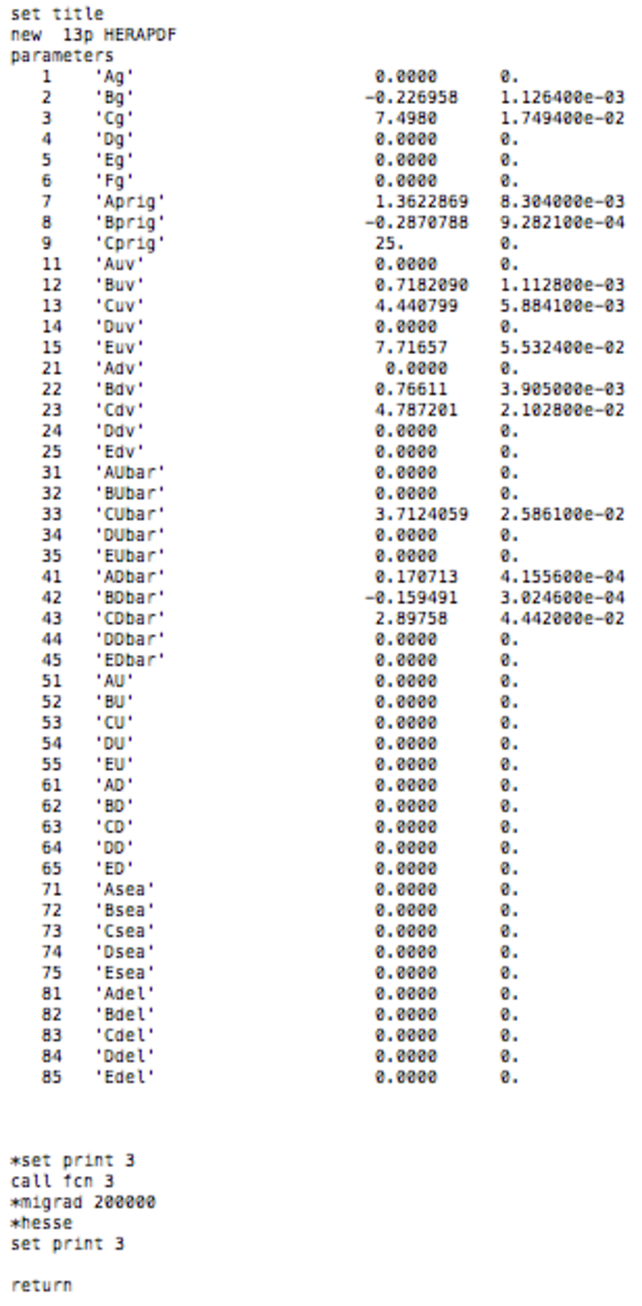
\includegraphics[width=0.45\linewidth]{figures/minuit.pdf}
\end{center}
\caption{An example of a minuit steering card.}
\label{fig:minuit}
\end{figure}

The first three lines set the title and specify the list of MINUIT parameters which are to follow.      
The index of parameters is the first column and it is hardwired to the source code:\\

\begin{tabular}{ll}
1 -10 & gluon parameters \\    
11-20 & uval  parameters \\
21-30 & dval  parameters \\
31-40 & Ubar  parameters \\
41-50 & Dbar  parameters \\
51-60 & U     parameters \\
61-70 & D     parameters \\
71-80 & Sea   parameters \\
81-90 &Delta parameters \\
91-100 & other parameters: alphas (95), fs=Dbar/str (96), fc=Ubar/ch (97)\\
\end{tabular}

The second column represents just user defined names,
the third column is  the input starting value for the parameter.
The forth column sets the step size (usually chosen the same order as the error).
If the step size is zero this parameter is FIXED.
The fifth column sets the lower bound of the fit parameter, 
The sixth column sets the upper bound of the fit parameter
if these columns are not filled then there are no bounds.

Only parameters that have non-zero stepsize are varied 
in the fit (free parameters). Another way to fix the parameters is
simply by typing at the end of the list of parameters ``FIX parameter number''.  
(make sure there is one line free before the minuit list).
Examples of commands taken by minuit are:\\

\begin{tabular}{ll}
call fcn 3  &   fit is not performed, only 1 iteration, useful for testing\\
            &    Minuit parameters ARE NOT minimized. \\
migrad       & fit is performed (default number of calls 2000).\\
migrad 20000 & fit is performed up to 20000 calls, then terminates.\\
hesse        & Hessian estimate of the \tt{MINUIT}\rm parameters \\
& (more reliable than \tt{MINUIT}\rm)\\
\end{tabular}


The output of the fit is stored in the output/ directory as \tt{minuit.out.txt}\rm.
Statements in minuit.out.txt which are useful for interpreting the results of the fit:
\begin{itemize}
\item \tt{FCN=575.16}\rm  \; this is total chisquare
\item \tt{FROM MIGRAD   STATUS=CONVERGED}\rm \; this is desirable for a fit that converged
\item \tt{FROM HESSE     STATUS=OK}\rm       \; this is desirable for a fit that converged 
\item \tt{ERROR MATRIX ACCURATE}   \rm       \; errors estimated with HESSE method
\end{itemize}

{\bf HERAFitter parameters for diffractive fits} \\
%%-----------------------------------------------------------
\label{sec:HFitterPar}

% minuit.in.txt
% ExtraMinimisationParameters

\begin{tabular}{l|l|l}
Parameter & HERAFitter name & input file\\
% \hline
$\Cini {\mathrm G}1$ & Ag & minuit.in.txt \\
$\Cini {\mathrm G}2$ & Bg & minuit.in.txt \\
$\Cini {\mathrm G}3$ & Cg & minuit.in.txt \\
$\Cini {\mathrm S}1$ & Auv & minuit.in.txt \\
$\Cini {\mathrm S}2$ & Buv & minuit.in.txt \\
$\Cini {\mathrm S}3$ & Cuv & minuit.in.txt \\
$\alpha_\Pom(0)$ & Pomeron\_a0 & steering.txt \\
$A_\Reg$ & Reggeon\_factor & steering.txt \\
$\alpha_\Reg(0)$ & Reggeon\_a0 & steering.txt \\
\end{tabular}
\vspace{0.7cm}

{\bf HERAFitter parameters for dipole fits} \\
The default  initial parameters for the fit without valence quarks are : 
\begin{table}[h]
\tiny
\begin{center}
\begin{tabular}{|c||c||c||c|c||c|c|c||c|c|} 
\hline 
$\sigma_0$ & $A_g$ & $\lambda_g$ & $C_g$ & $cBGK$& $eBGK$\\
\hline
37.490 & 3.3446 & 0.0298 & 2.6302 & 4.0 & 15.362 \\
\hline
\end{tabular}
\end{center}
\end{table}
\\
For the BGK dipole model fits with valence quarks the initial parameters and the obtained $\chi^2$ are:

\begin{table}[ht]
\begin{center}
\begin{tabular}{|c||c||c||c|c||c|c|c||c|c|c||c|}
\hline
No&
$Q^2$&&
$\sigma_0$ & $A_g$ & $\lambda_g$ & $C_g$ & $C_{BGK}$& $\mu_{0}^2$& $Np$&
$\chi^2/Np$\\
\hline
1 &
$Q^2 \ge 3.5$ &  LO & 66.6 & 4.0 & -0.039 & 18.6& 4.0 & 5.3  & 196 &  0.930 \\
\hline
2 &
$Q^2 \ge 3.5$ & NLO & 79.4 & 3.2 &-0.021 & 13.7 & 4.0 & 6.7 & 196 & 0.927 \\
\hline
\end{tabular}
\end{center}
\end{table}
\end{description}


%%%%%%%%%%%%%%%%%%%%%%%%%%%%%%%%%%%%%%%%
\subsubsection{Data file format}
\label{sec:dataformat}
   Experimental data are provided by the standard {\tt ASCII} text files. The files
   contain a "header" which describes the data format and the "data" in terms
   of a  table. Each line of the data table corresponds to a
   data point, the meaning of the columns is specified in the file header.

   For example, a header for HERA-I combined H1-ZEUS data for e+p neutral 
   current scattering cross section is given in the file

\begin{verbatim}
       datafiles/H1ZEUS_NC_e-p_HERA1.0.dat
\end{verbatim}

   The format of the file follows standard "namelist" conventions. Comments 
   start with an exclamation mark.  Pre-defined variables are:
\begin{itemize}
     \item{\tt Name}        --- (string) provides the name of the data set
    \item{\tt  Reaction}    --- (string) reaction type of the data set. Reaction type is used 
                      to trigger the corresponding theory calculation. The following 
                      reaction types  are currently supported by the HERAFitter:
                      \begin{itemize}
                        \item {\tt 'NC e+-p'}  -- double differential NC ep scattering
                                      (ZM-VFNS and RT-VFNS schemes) 
                        \item {\tt 'CC e+-p'}  -- double differential CC ep scattering
                                      (ZM-VFNS scheme)
                        \item {\tt 'CC pp'}    -- single differential $d \sigma_{W^{\pm}}/d eta_{\ell^{\pm}}$
                                      production and W asymmetry at $pp$ and $p\bar{p}$ 
                                      colliders (LO+kfactors and APPLGRID interface)
                        \item {\tt 'NC pp'}    -- single differential $d \sigma_Z / d y_Z$ at $pp$ and
                                      $p\bar{p}$ colliders
                                      ({\tt LO} with k-factors and {\tt APPLGRID} interface)

                        \item 'pp jets APPLGRID' -- $pp\to$ inclusive jet production, using
                                     {\tt APPLGRID}

                        \item 'FastNLO jets' -- jet cross sections using {\tt FastNLO} interface.
                                     All $ep$, $pp$ and $p\bar{p}$ colliders are supported.

                        \item 'FastNLO ep jets normalised' -- jet cross sections in the $ep$ collisions 
                                     using {\tt FastNLO} interface and normalised to the inclusive DIS cross sections.

                      \end{itemize}                       
      \item {\tt NData}       --- (integer) specifies number of data points in the file. 
                     This corresponds to the number of table rows which 
                     follow after the header.
      \item {\tt NColumn}     --- (integer) number of columns in the data table.
      \item {\tt ColumnType}  --- (array of strings)
                      Defines layout of the data table. The following column types
                      are pre-defined: 'Bin', 'Sigma', 'Error' and 'Dummy'
                      The keywords are case sensitive. 'Bin' correspond to an
                      abstract bin definition, 'Sigma' corresponds to the data
                      measurement, 'Error' - to various type of uncertainties and
                      'Dummy' indicates that the column should be ignored.
      \item {\tt ColumnName}  --- (array of strings)
                      Defines names of the columns. The meaning of the name depends
                      on the ColumnType. For ColumnType 'Bin', ColumnName gives a
                      name of the abstract bin. The abstract bins can contain
                      any variable names, but some of them must be present for 
                      correct cross section calculation. For example, 'x', 'Q2' and
                      'y' are required for DIS NC cross-section calculation.
 
                      For ColumnType 'Sigma', ColumnName provides a label for 
                      the observable, which can be any string.
 
                      For ColumnType 'Error', the following names have special meaning:
                      \begin{itemize}
                       \item 'stat'  -- specifies column with statistical uncertainties, request Poisson re-scaling;
                       \item 'stat const'  -- specifies column with statistical uncertainties, request no re-scaling of the errors;
                       \item 'uncor' -- specifies column with uncorrelated uncertainties. Any name containing keyword ``uncor'' is treated as an uncorrelated
  error source, e.g. ``h1 uncor'';  
                       \item 'uncor const' -- specifies column with uncorrelated uncertainties, request no re-scaling of the errors;  
                       \item 'total' -- specifies column with total uncertainties. 
                                  Total uncertainties are not used in the fit,
                                  however there is an additional check is performed
                                  if 'total' column is specified: sum in quadrature
                                  of statistical, uncorrelated and correlated 
                                  systematic uncertainties is compared to the total
                                  and a warning is issued if they differ significantly.
                       \item'ignore' - specifies column to be ignored (for special studies).
                       \item Other names specifies columns of correlated systematic 
                      uncertainty. For a given data file, each column of the correlated
                      uncertainty must have unique name. To specify correlation across
                      data files, same name must be used for different files.  
                      \end{itemize}
      \item {\tt SystScales}  --- (array of float)
                      For special studies, systematic uncertainties can be scaled
                      The numbering of uncertainties starts from the first column
                      with the ColumnType 'Error'. For example, setting 
\begin{verbatim}
                  SystScale(1) = 2.  
\end{verbatim}
                      in {\tt datafiles/H1ZEUS\_NC\_e-p\_HERA1.0.dat} would scale systematic 
                      uncertainty by factor of two.                       
      \item {\tt Percent}     --- (array of bool) For each uncertainty specify if it is given in 
                      absolute ("false") or in percent ("true").  The numbering of 
                      uncertainties starts from the first column with the 
                      {\tt ColumnType} 'Error' (see example above).
      \item {\tt NInfo}       --- (integer) Calculation of the cross-section predictions may 
                      require  additional information about the data set. The number of 
                      information strings is given by NInfo
      \item {\tt CInfo}       --- (array of strings) Names of the information strings. 
                      Several of them are predefined for different cross-section 
                      calculations.
      \item {\tt DataInfo}    --- (array of float) Values, corresponding to {\tt CInfo} names.
      \item {\tt IndexDataset} -- (integer) Internal \fitter\ index of the data set. Provide unique
                      numbers to get extra info for $\chi^2/dof$ for each data set.      
      \item {\tt TheoryInfoFile} --- (string) Optional additional theory file with extra 
                     information for cross-section calculation. This could be k-factors,
                     {\tt APPLGRID} file or {\tt FastNLO} table.  
      \item {\tt TheoryType} --- (string) Theory file type ('kfactor', 'applgrid' or 'fastnlo').      
      \item {\tt NKFactor}   --- (integer) For kfactor files, number of columns in
                     {\tt TheoryInfoFile}.
      \item {\tt KFactorNames} --- (array of strings) For kfactor files, names of columns in 
                     {\tt TheoryInfoFile}.
\end{itemize}

Depending on the chosen process specific requirements for the header might be present. 
Dataset-wise options are provided by a {\tt CInfo} / {\tt DataInfo} variable set. In case the information
varies between data points (e.g. bin borders, hadronisation corrections etc.) it is
provided in the data file and recognised by the program using reserved column names.
In the following all these requirements are listed and briefly explained.

%%%%%%%%%%%%%%%%%%%%%%%%%%%%%%%%%%%%%%%%
\begin{description}
\item \bf{Data format requirements for DIS}\rm

In this subsection we describe specific requirements for files using 'NC e+-p' and 'CC e+-p'
reaction types. Examples of such input files are:

{\tt datafiles/H1ZEUS\_NC\_e-p\_HERA1.0.dat}

{\tt datafiles/H1ZEUS\_CC\_e-p\_HERA1.0.dat}.

The properly formatted DIS input files will have the following fields available
in the {\tt CInfo} variable list: 

\begin{itemize} 
    \item  {\tt 'sqrt(S)'} --- the ep collision centre-of-mass energy in GeV. In particular, for 
    HERA based results the the corresponding {\tt DataInfo} value should be $300.$ for measurements
    based on data collected prior to $1997$ (inclusive) and $318.$ for data collected after 1997.
    
    \item {\tt 'reduced'} --- a field indicating whether calculated cross section should be reduced (1.) or not (0.)
    (reference to proper equation somewhere in this manual).
    
    \item {\tt 'e charge'} --- electric charge of the colliding lepton beam. Supported {\tt DataInfo} values
    are '1.' for electron and '-1.' for positron.

    \item {\tt 'e polarity'} --- polarity of the lepton beam. The corresponding {\tt DataInfo} value 
    should be between $-1.0$ and $1.0$ (is this true?) with abs($1.0$) indicating fully polarised
    beam and $0.0$ fully unpolarised one. 

    In case of non-vanishing polarity the following additional fields are required:

    \item {\tt 'pol err unc'} --- explain

    \item {\tt 'pol err corLpol'} --- explain
 
    \item {\tt 'pol err corTpol'} --- explain

\end{itemize}

The inclusive DIS cross sections are calculated on an x-Q$^2$-y grid. Correspondingly,
the following columns need to present in the correctly formatted input file: 
{\tt 'x'}, {\tt 'Q2'} and {\tt 'y'}.


%%%%%%%%%%%%%%%%%%%%%%%%%%%%%%%%%%%%%%%%

\item \bf{Data format requirements for FastNLO} \rm

In this subsection we describe data format specific for the FastNLO implementation
accessed by choosing 'FastNLO jets' and 'FastNLO ep jets normalised' reaction types.
Examples of properly formatted files are:

   {\tt datafiles/HERA/ZEUS\_InclJets\_HighQ2\_98-00.dat}

   {\tt datafiles/HERA/H1\_NormInclJets\_HighQ2\_99-07.dat}.

{\tt TheoryType = 'FastNLO'} indicates usage of the FastNLO. The variable {\tt ThoryInfoFile} 
should contain the proper path to the FastNLO table in version 2.0 or higher.
\fitter\ supports both flexible and inflexible scales.
Older FastNLO tables can be still accessed through the APPLGRID interface.

The following fields are required to be present in the {\tt CInfo} list:

\begin{itemize}

    \item {\tt 'PublicationUnits'} --- The desired units in which the cross sections 
    are calculated by the FastNLO code. If the corresponding {\tt DataInfo} field is 
    set to '1.' the cross sections will be given in the same units as used in the
    relevant publication. In the case it is set to '0.', absolute cross section
    units will be used. 

    \item {\tt 'MurDef', 'MufDef'} --- The renormalisation and factorisation scale definitions
    used with variable scale FastNLO tables. If the chosen FastNLO table does not support 
    variable scales, these fields will be ignored and the scale embedded within the table will 
    be used instead. The values of the corresponding {\tt DataInfo} fields set 
    the renormalisation scale $\mu_r$ and factorisation scale $\mu_f$ following the FastNLO standard:
    \begin{align*} 
       \text{value} :&\quad \text{definition} \\
       0 :&\quad   \mu_{r/f}^2 = \mu_1^2 \\
       1 :&\quad   \mu_{r/f}^2 = \mu_2^2 \\
       2 :&\quad   \mu_{r/f}^2 = ( \mu_1^2 + \mu_2^2 )\\
       3 :&\quad   \mu_{r/f}^2 = ( \mu_1^2 + \mu_2^2 ) / 2 \\
       4 :&\quad   \mu_{r/f}^2 = ( \mu_1^2 + \mu_2^2 ) / 4 \\
       5 :&\quad   \mu_{r/f}^2 = (( \mu_1 + \mu_2 ) / 2 )^2\\
       6 :&\quad   \mu_{r/f}^2 = (( \mu_1 + \mu_2 ))^2\\
       7 :&\quad   \mu_{r/f}^2 = \text{max}( \mu_1^2, \mu_2^2)\\
       8 :&\quad   \mu_{r/f}^2 = \text{min}( \mu_1^2, \mu_2^2) \\
       9 :&\quad   \mu_{r/f}^2 = (\mu_1 * exp(0.3 * \mu_2)) ^2
   \end{align*}

   where $\mu_1$ and $\mu_2$ are specific scales chosen during production of the table. In particular
   for jet production at HERA traditionally 
   \begin{equation*}
          \mu_1^2 = Q^2 \quad \quad \quad \mu_2^2 = p_T^2
    \end{equation*}  

   \item {\tt sqrt(S)} --- Should be defined only for 'FastNLO ep jets normalised' reaction type. 
         The ep collision centre-of-mass energy in GeV. In particular, for 
         HERA based results the the corresponding {\tt DataInfo} value should be $300.$ for measurements
         based on data collected prior to $1997$ (inclusive) and $318.$ for data collected after 1997.

   \item {\tt 'lumi(e-)/lumi(tot)'} --- Should be defined only for 'FastNLO ep jets normalised'
         reaction type. The normalisation depends on the ratio of the luminosities of the positron and electron data 
         used for the cross section measurement. This ratio should  be
         given in a format (lumi($e^-$) / (lumi($e^-$) + lumi($e^+$)) and ashould take values between [0., 1.].

   \item {\tt 'UseZMVFNS'} --- Should be defined for 'FastNLO ep jets normalised' reaction type. The calculation
         of the integrated inclusive DIS cross sections could be time consuming.
         This option provides an opportunity to use a "Zero Mass Variable Flavour
         Number Scheme" approximation which is very fast and provides
         enough precision for normalisation purposes. ZMVNS is used if 
         the corresponding {\tt DataInfo} field is set to 1. Otherwise, the same scheme
         is used as defined globally with the variable 'HF\_SCHEME' defined in steering.txt file.
\end{itemize}


In addition there are some specific values within the {\tt ColumnName} field which allow
information specific to each data point to be passed. They are listed below:

\begin{itemize}
     \item{\tt 'Z0Corr'} --- (optional) The correction due to the $Z_0$ boson exchange.
                 If it is given, each point calculated by the FastNLO code will be
                 multiplied by the {\tt Z0Corr} value.

     \item{\tt 'NPCorr'} --- (optional) The non-perturbative correction.
                 If it is given, each point calculated by the FastNLO code will be
                 multiplied by the {\tt NPCorr} value. {\tt Z0Corr} and {\tt NPCorr} can be added 
                 simultaneously, and in this case the calculated cross sections
                 will be multiplied by the product {\tt Z0Corr} * {\tt NPCorr}.

    \item{\tt 'q2min', 'q2max', 'ymin', 'ymax', 'xmin', 'xmax'} --- Should be defined for 
         'FastNLO ep jets normalised' reaction type and are used to define 
         DIS phase space for the normalisation. Since these three ({\tt q2, y, x}) are 
         connected by the relation
         \begin{equation}
              Q^2 = x \cdot y \cdot s
         \end{equation}
         only two are required to be present to unambiguously define the DIS phase space for each data point.
        
\end{itemize}
\end{description}


%%%%%%%%%%%%%%%%%%%%%%%%%%%%%%%%%%%%%%%%
\subsubsection{Understanding the output}
  The results of the minimization are printed to the standard output and written
  to files in the {\tt output/} directory. 

  The quality of the fit can be judged based on the total $\chi^2$ per degrees of freedom.
  It is printed for each iteration as 
\begin{verbatim}
                      Iteration   Chi2   NDF       Chi2/NDF
   FitPDF f,ndf,f/ndf      3      588.64 579        1.02
\end{verbatim}
  The resulting $\chi^2$ is reported at the end of minimisation for each data set and for the correlated 
  systematic uncertainties separately. This information is printed and written
  to the {\tt output/Results.txt} file. The {\tt Results.txt} file contains additional 
  information about shifts of the correlated systematic uncertainties.

  The minimization information from the {\tt minuit} program is stored using the standard {\tt minuit} output format in the {\tt output/minuit.out.txt}
  file. The level of verbosity for this information can be changed by {\tt minuit} commands
  in the {\tt minuit.in.txt} file. 
  It is a good idea to check that minuit does not report any errors
  or warnings at the end of minimisation.
  
  Point by point comparison of the data and predictions after the minimization 
  is provided in the file stored in {\tt output/fittedresults.txt}. The file reports three columns
  corresponding to the three first bins of the input tables, data value, sum in 
  quadrature of statistical and uncorrelated systematic uncertainty, total
  uncertainty and then the predicted value, before and after applying correlated systematic shifts,
  the pull between the  data and theory and 
  the data set index. The pull $p$ is calculated as 
  \begin{equation}
      p = \frac{ \mu - m} {\sigma_{\rm uncor}}
  \end{equation}
  where $\mu$ is the data value, $m$ is the prediction and $\sigma_{\rm uncor}$ is the total
  uncorrelated uncertainty.
  Similar information is stored in the {\tt pulls.first.txt} and {\tt pulls.last.txt} files
  ( dataset index, first bin, second bin, third bin, theory, data, pull).
  Theory is  adjusted for systematic error shifts in this case.

  The output PDFs are stored in  {\tt output/pdfs\_q2val\_XX.txt} files.
  Each of the files reports values of gluon, and quark PDFs as a function of $x$
  for fixed $Q^2$ points. The $Q^2$ values and $x$ grid are specified by 
  {\tt \&Output} namelist in the {\tt steering.txt} file.
  
  The PDF information and data to theory comparisons can be plotted using 
  the {\tt bin/DrawResults} program.  Calling it without arguments plots results from the
  {\tt output/} directory. Giving the programme one argument specifies the sub-directory 
  where the information is read. Calling the {\tt bin/DrawResults} program with two
  arguments provides a comparison of the PDFs obtained in the two fits.
  
  In addition the \fitter\ package provides PDFs in the {\tt LHAPDF} format as {\tt output/lhapdf.block.txt} file. 
  To obtain the
  {\tt LHAPDF} grid file, run the {\tt tools/tolhapdf.cmd} script. The script provides a
  {\tt PDFs.LHgrid} file which can be read by the lhapdf version lhapdf-5.8.6.tar.gz
  or later.
%%%%%%%%%%%


